\begin{figure}[H]
\centering
\includegraphics[page=4,width=0.33\textwidth]{\FCNCFigures/xTFW/showFake/NOMINAL/reg2mtau1b2jos_vetobtagwp70_highmet/BDTG_test.pdf}
\put(-40, 90){\textbf{(a1)}}
\includegraphics[page=5,width=0.33\textwidth]{\FCNCFigures/xTFW/showFake/NOMINAL/reg2mtau1b2jos_vetobtagwp70_highmet/BDTG_test.pdf}
\put(-40, 90){\textbf{(a2)}}
\includegraphics[width=0.33\textwidth]{\FCNCFigures/xTFW/BDT/roc_reg2mtau1b2jos.pdf}
\put(-70, 90){\textbf{(a3)}}\\
\includegraphics[page=4,width=0.33\textwidth]{\FCNCFigures/xTFW/showFake/NOMINAL/reg2mtau1b3jos_vetobtagwp70_highmet/BDTG_test.pdf}
\put(-40, 90){\textbf{(b1)}}
\includegraphics[page=5,width=0.33\textwidth]{\FCNCFigures/xTFW/showFake/NOMINAL/reg2mtau1b3jos_vetobtagwp70_highmet/BDTG_test.pdf}
\put(-40, 90){\textbf{(b2)}}
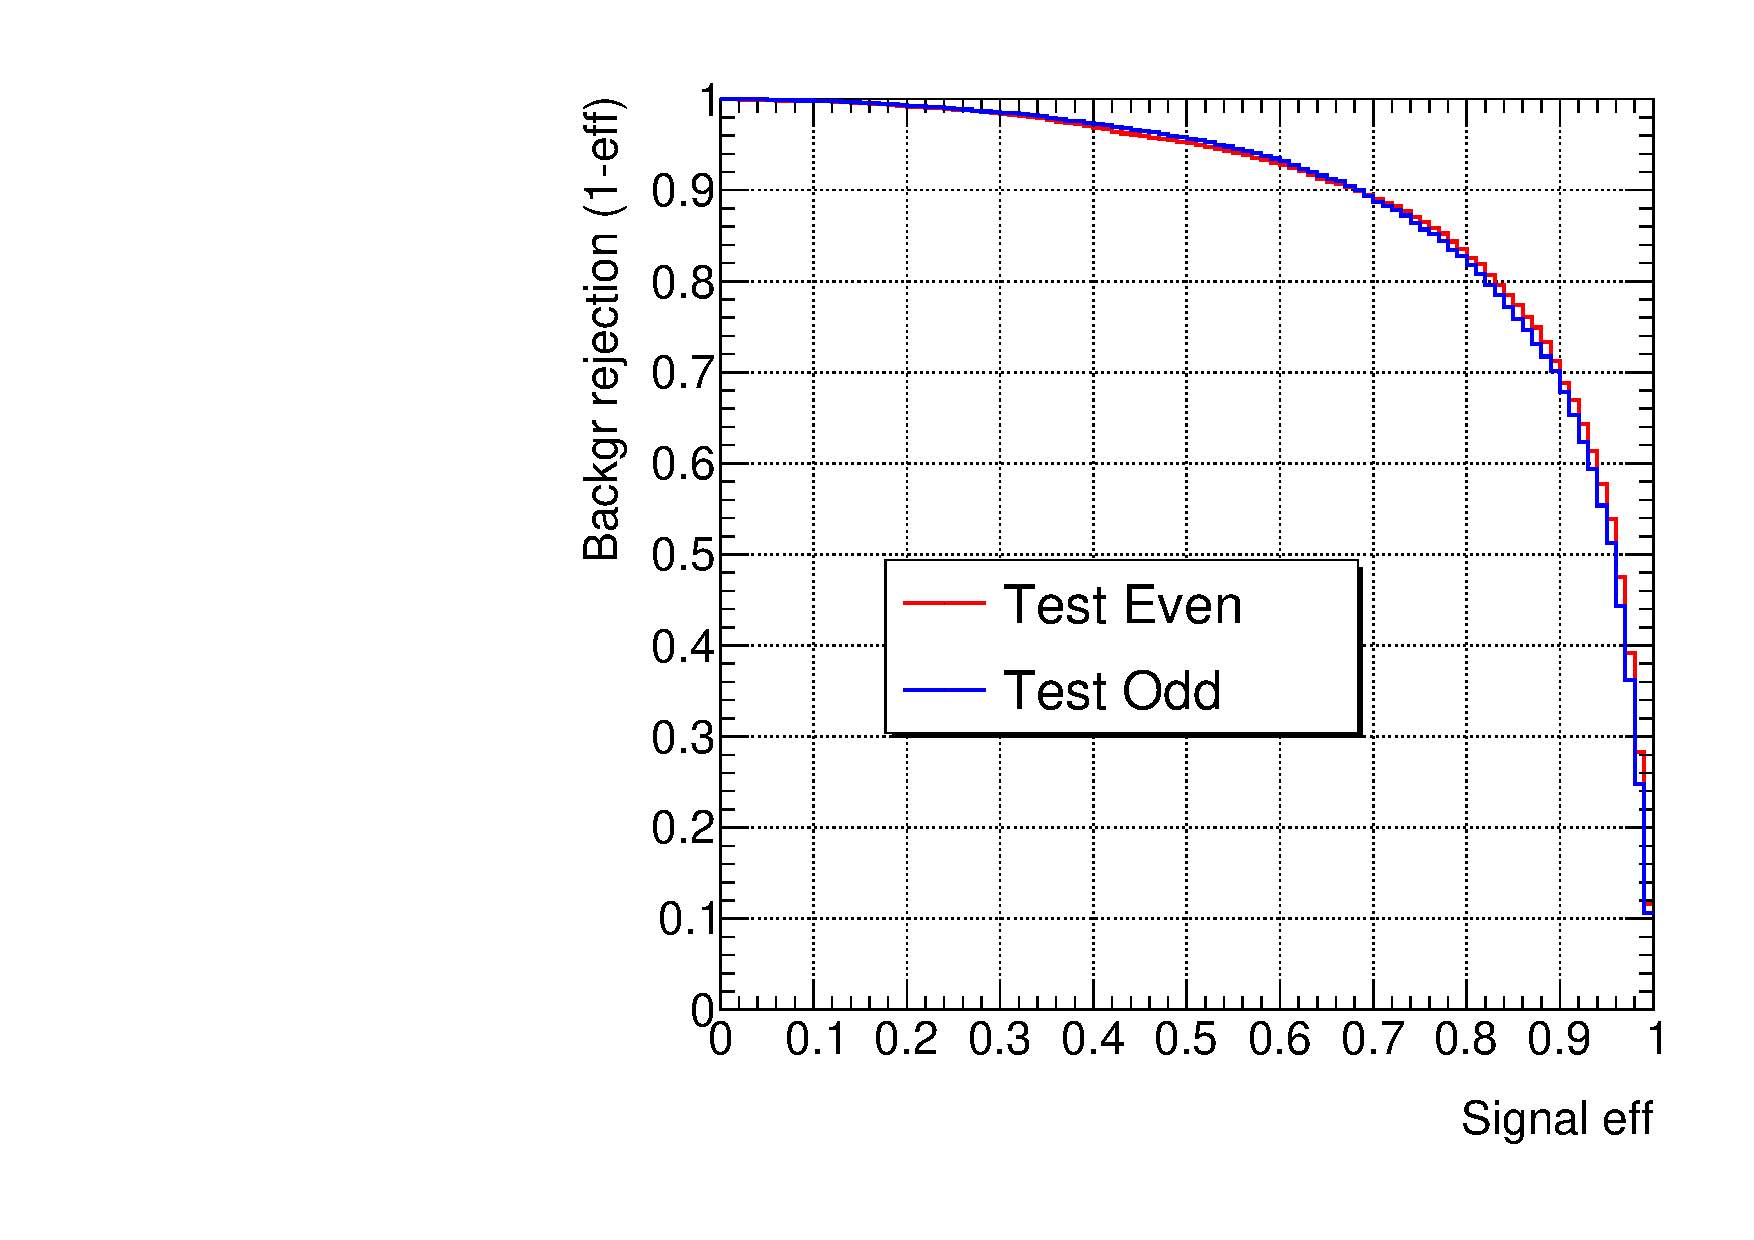
\includegraphics[width=0.33\textwidth]{\FCNCFigures/xTFW/BDT/roc_reg2mtau1b3jos.pdf}
\put(-70, 90){\textbf{(b3)}}\\
\includegraphics[page=7,width=0.33\textwidth]{\FCNCFigures/xTFW/showFake/NOMINAL/reg2mtau1b2jos_vetobtagwp70_highmet/BDTG_test.pdf}
\put(-40, 90){\textbf{(c1)}}
\includegraphics[page=7,width=0.33\textwidth]{\FCNCFigures/xTFW/showFake/NOMINAL/reg2mtau1b3jos_vetobtagwp70_highmet/BDTG_test.pdf}
\put(-40, 90){\textbf{(c2)}}\\
\caption{ The BDT output distributions for the background and TT signal (a1, b1), background and ST signal (a2, b2), background and different types of signals (c1,c2) and ROC curves (a3, b3) in the $t_h\thadhad$-2j (a1-3,c1), $t_h\thadhad$-3j (b1-3,c2) regions of leptonic channel. Only statistical uncertainties are being shown. Underflow and overflow bins are included respectively in the first and last bins. Empty data bins here are always blinded based on our strategy.The real tau contributions shown from various MC samples.}% The Kolmogorov Test values for the training and testing BDT distributions are also indicated.
\label{fig:overtrain_hadhad}
\end{figure}

\begin{figure}[H]
\centering
\includegraphics[page=4,width=0.33\textwidth]{\FCNCFigures/tthML/showFake/faketau/postfit/NOMINAL/reg1l1tau1b2j_os_vetobtagwp70_highmet/BDTG_test.pdf}
\put(-40, 80){\textbf{(a1)}}
\includegraphics[page=5,width=0.33\textwidth]{\FCNCFigures/tthML/showFake/faketau/postfit/NOMINAL/reg1l1tau1b2j_os_vetobtagwp70_highmet/BDTG_test.pdf}
\put(-40, 80){\textbf{(a2)}}
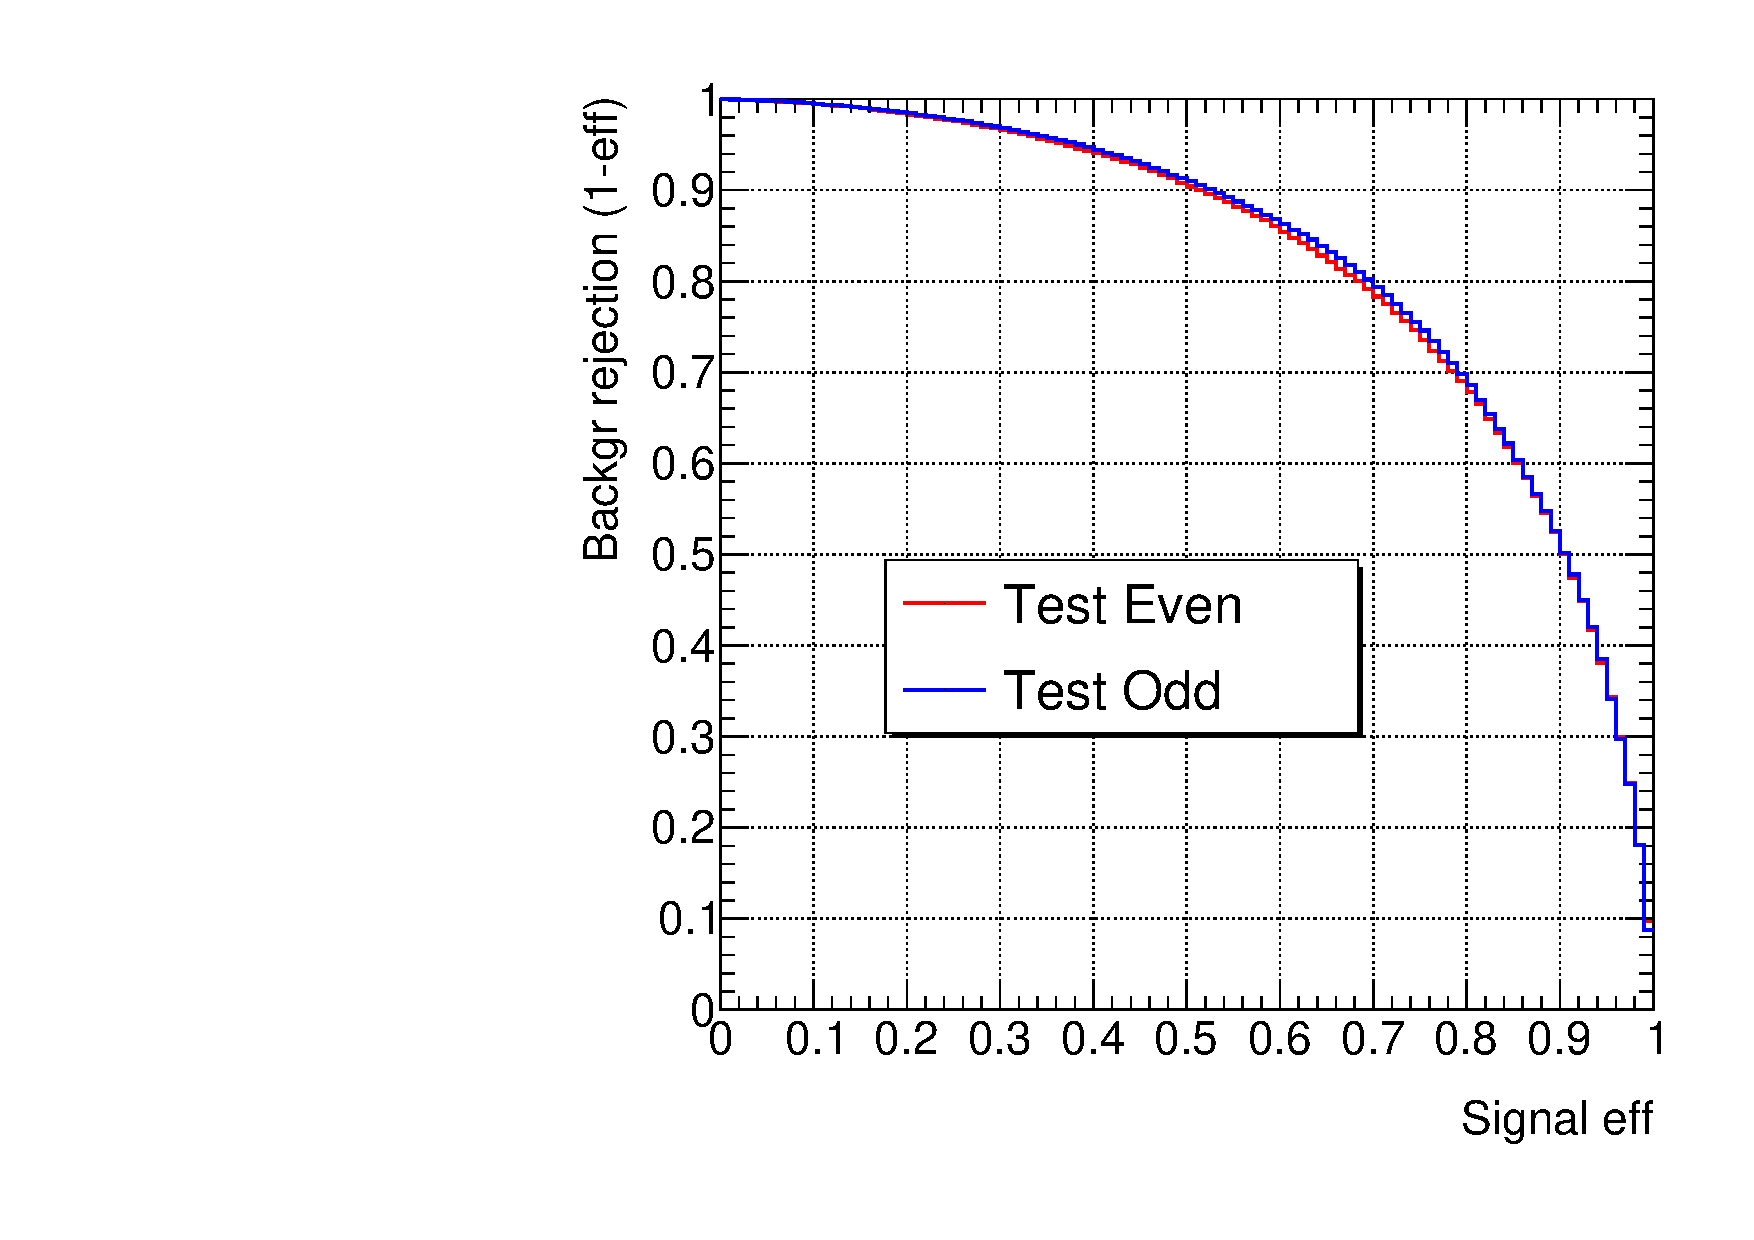
\includegraphics[width=0.33\textwidth]{\FCNCFigures/tthML/BDT/roc_reg1l1tau1b2j_os.pdf}
\put(-70, 85){\textbf{(a3)}}\\
\includegraphics[page=4,width=0.33\textwidth]{\FCNCFigures/tthML/showFake/faketau/postfit/NOMINAL/reg1l1tau1b3j_os_vetobtagwp70_highmet/BDTG_test.pdf}
\put(-40, 80){\textbf{(b1)}}
\includegraphics[page=5,width=0.33\textwidth]{\FCNCFigures/tthML/showFake/faketau/postfit/NOMINAL/reg1l1tau1b3j_os_vetobtagwp70_highmet/BDTG_test.pdf}
\put(-40, 80){\textbf{(b2)}}
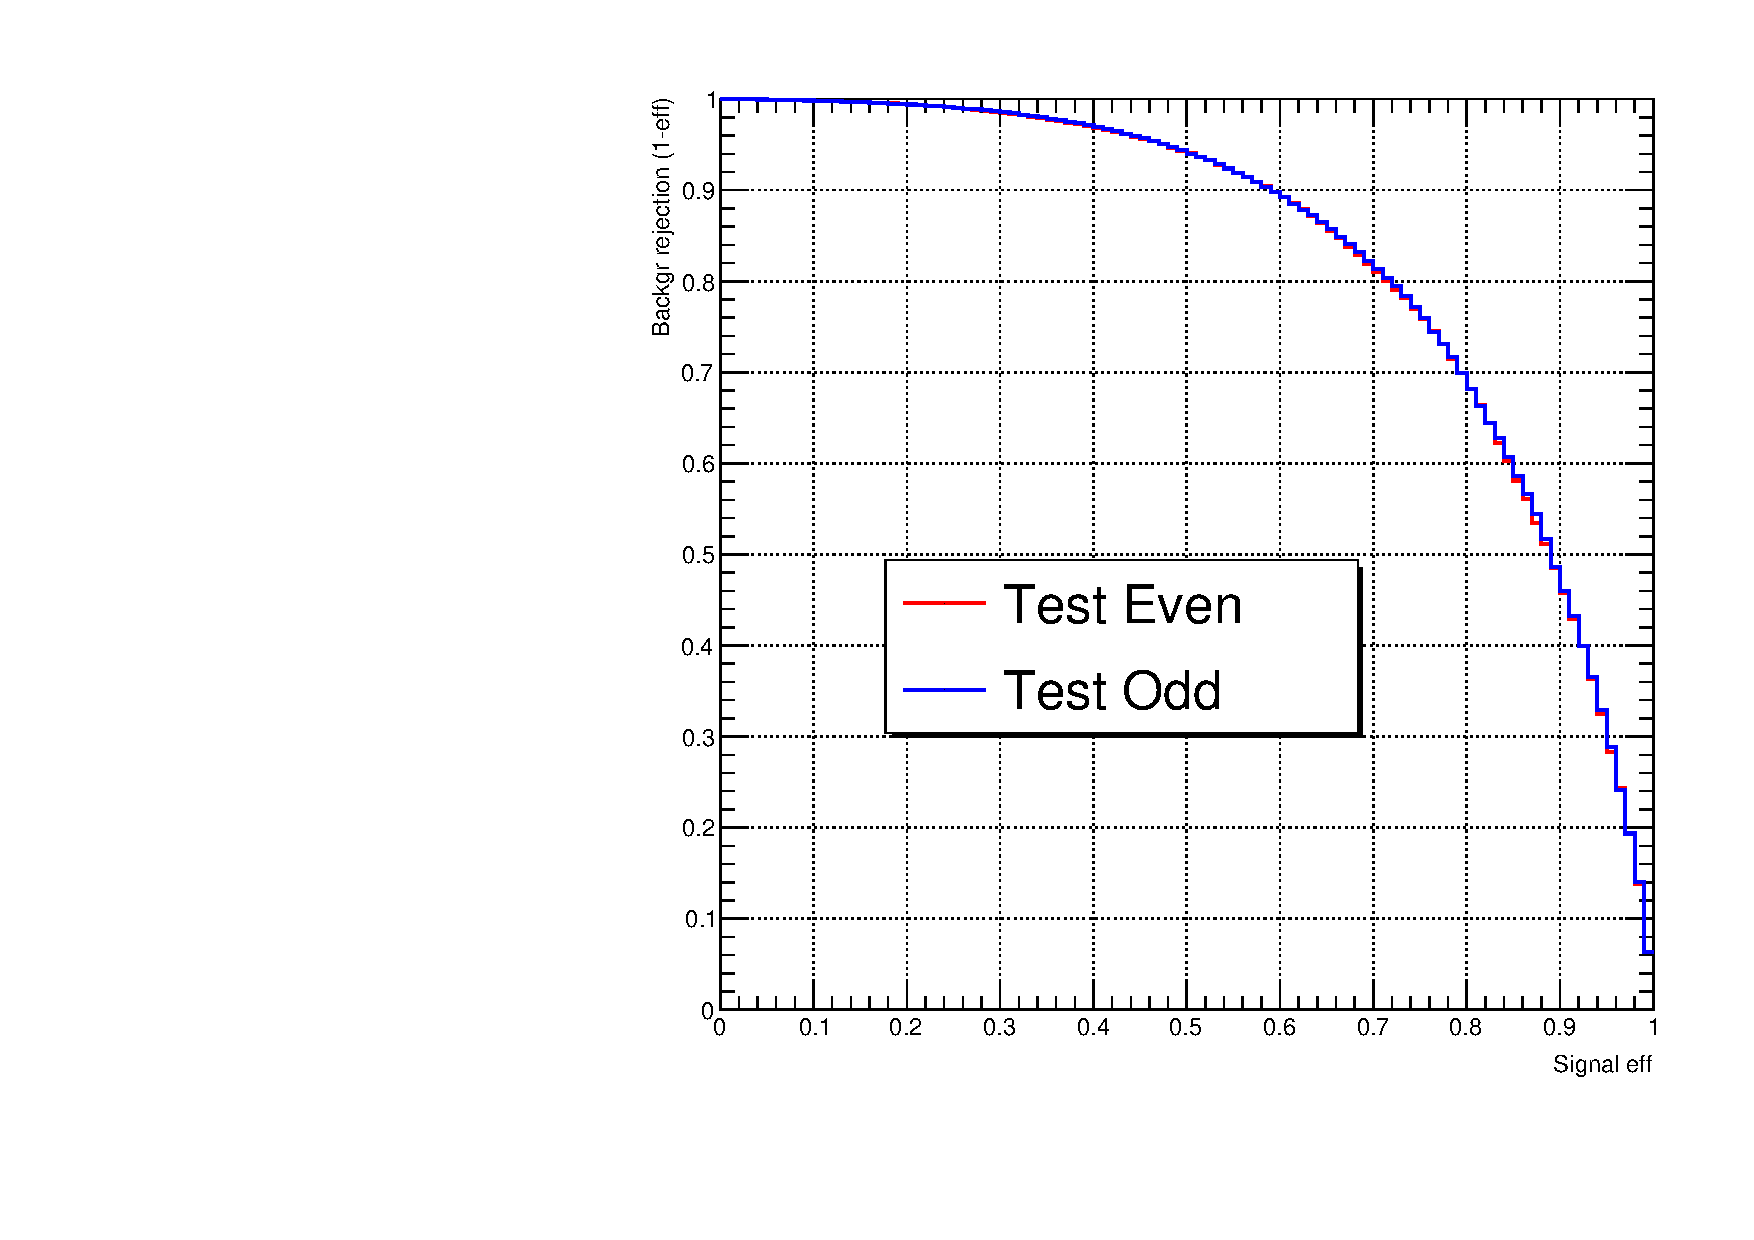
\includegraphics[width=0.33\textwidth]{\FCNCFigures/tthML/BDT/roc_reg1l1tau1b3j_os.pdf}
\put(-70, 85){\textbf{(b3)}}\\
\includegraphics[page=9,width=0.33\textwidth]{\FCNCFigures/tthML/showFake/faketau/postfit/NOMINAL/reg1l1tau1b2j_os_vetobtagwp70_highmet/BDTG_test.pdf}
\put(-40, 80){\textbf{(a1)}}
\includegraphics[page=9,width=0.33\textwidth]{\FCNCFigures/tthML/showFake/faketau/postfit/NOMINAL/reg1l1tau1b3j_os_vetobtagwp70_highmet/BDTG_test.pdf}
\put(-40, 80){\textbf{(b1)}}\\
\caption{ The BDT output distributions for the background and TT signal (a1, b1), background and ST signal (a2, b2), background and different types of signals (c1,c2) and ROC curves (a3, b3) in the $t_h\tlhad$-2j (a1-3,c1), $t_h\tlhad$-3j (b1-3,c2) regions of leptonic channel.Only statistical uncertainties are being shown. Underflow and overflow bins are included respectively in the first and last bins. Empty data bins here are always blinded based on our strategy. The real tau contributions shown from ttbar and other MC including diboson, single top, and V+jets.  }% The Kolmogorov Test values for the training and testing BDT distributions are also indicated.
\label{fig:overtrain_lephad}
\end{figure}
\begin{figure}[H]
\centering
\includegraphics[page=4,width=0.33\textwidth]{\FCNCFigures/tthML/showFake/faketau/postfit/NOMINAL/reg1l2tau1bnj_os/BDTG_test.pdf}
\put(-40, 80){\textbf{(a1)}}
\includegraphics[page=5,width=0.33\textwidth]{\FCNCFigures/tthML/showFake/faketau/postfit/NOMINAL/reg1l2tau1bnj_os/BDTG_test.pdf}
\put(-40, 80){\textbf{(a2)}}
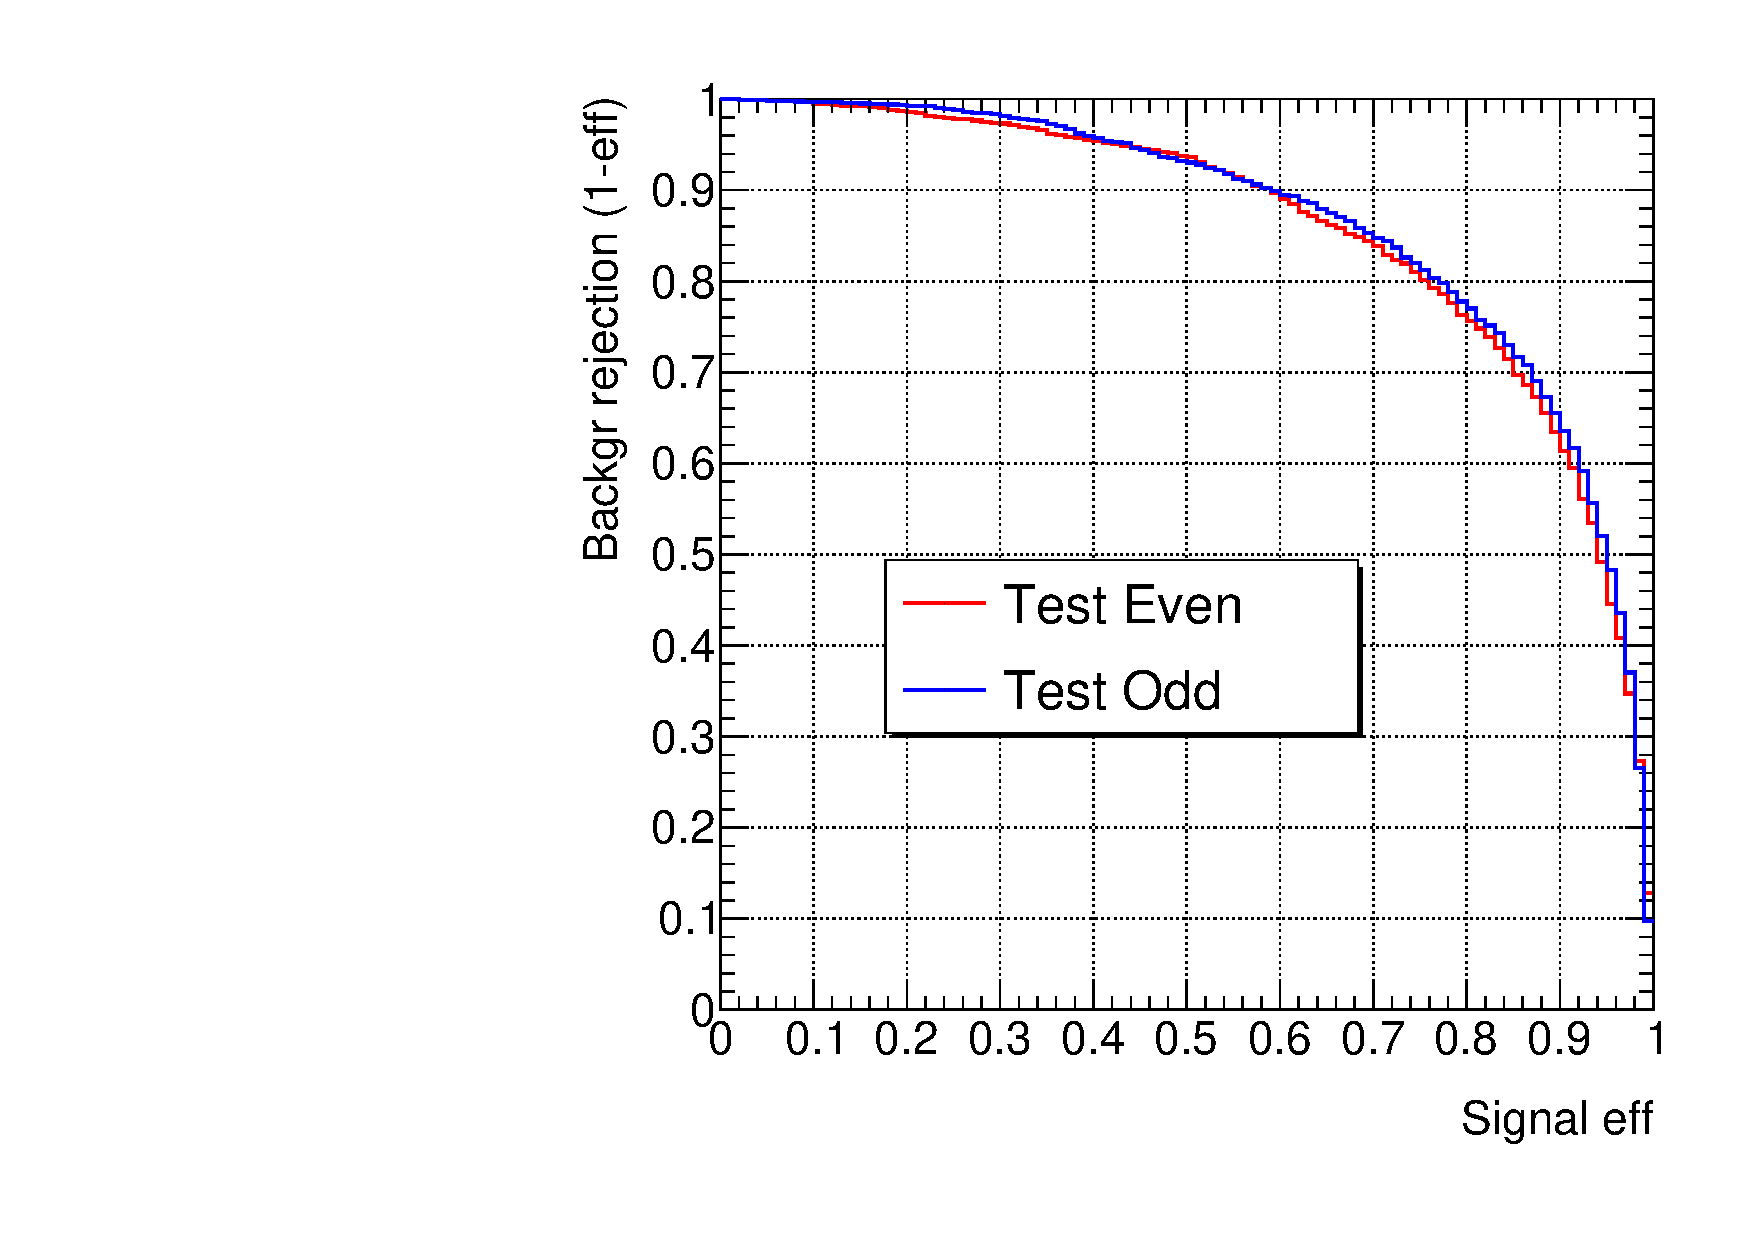
\includegraphics[width=0.33\textwidth]{\FCNCFigures/tthML/BDT/roc_reg1l2tau1bnj_os.pdf}
\put(-70, 85){\textbf{(a3)}}\\

\includegraphics[page=4,width=0.33\textwidth]{\FCNCFigures/tthML/showFake/faketau/postfit/NOMINAL/reg1l1tau1b1j_ss_vetobtagwp70_highmet/BDTG_test.pdf}
\put(-40, 80){\textbf{(b1)}}
\includegraphics[page=5,width=0.33\textwidth]{\FCNCFigures/tthML/showFake/faketau/postfit/NOMINAL/reg1l1tau1b1j_ss_vetobtagwp70_highmet/BDTG_test.pdf}
\put(-40, 80){\textbf{(b2)}}
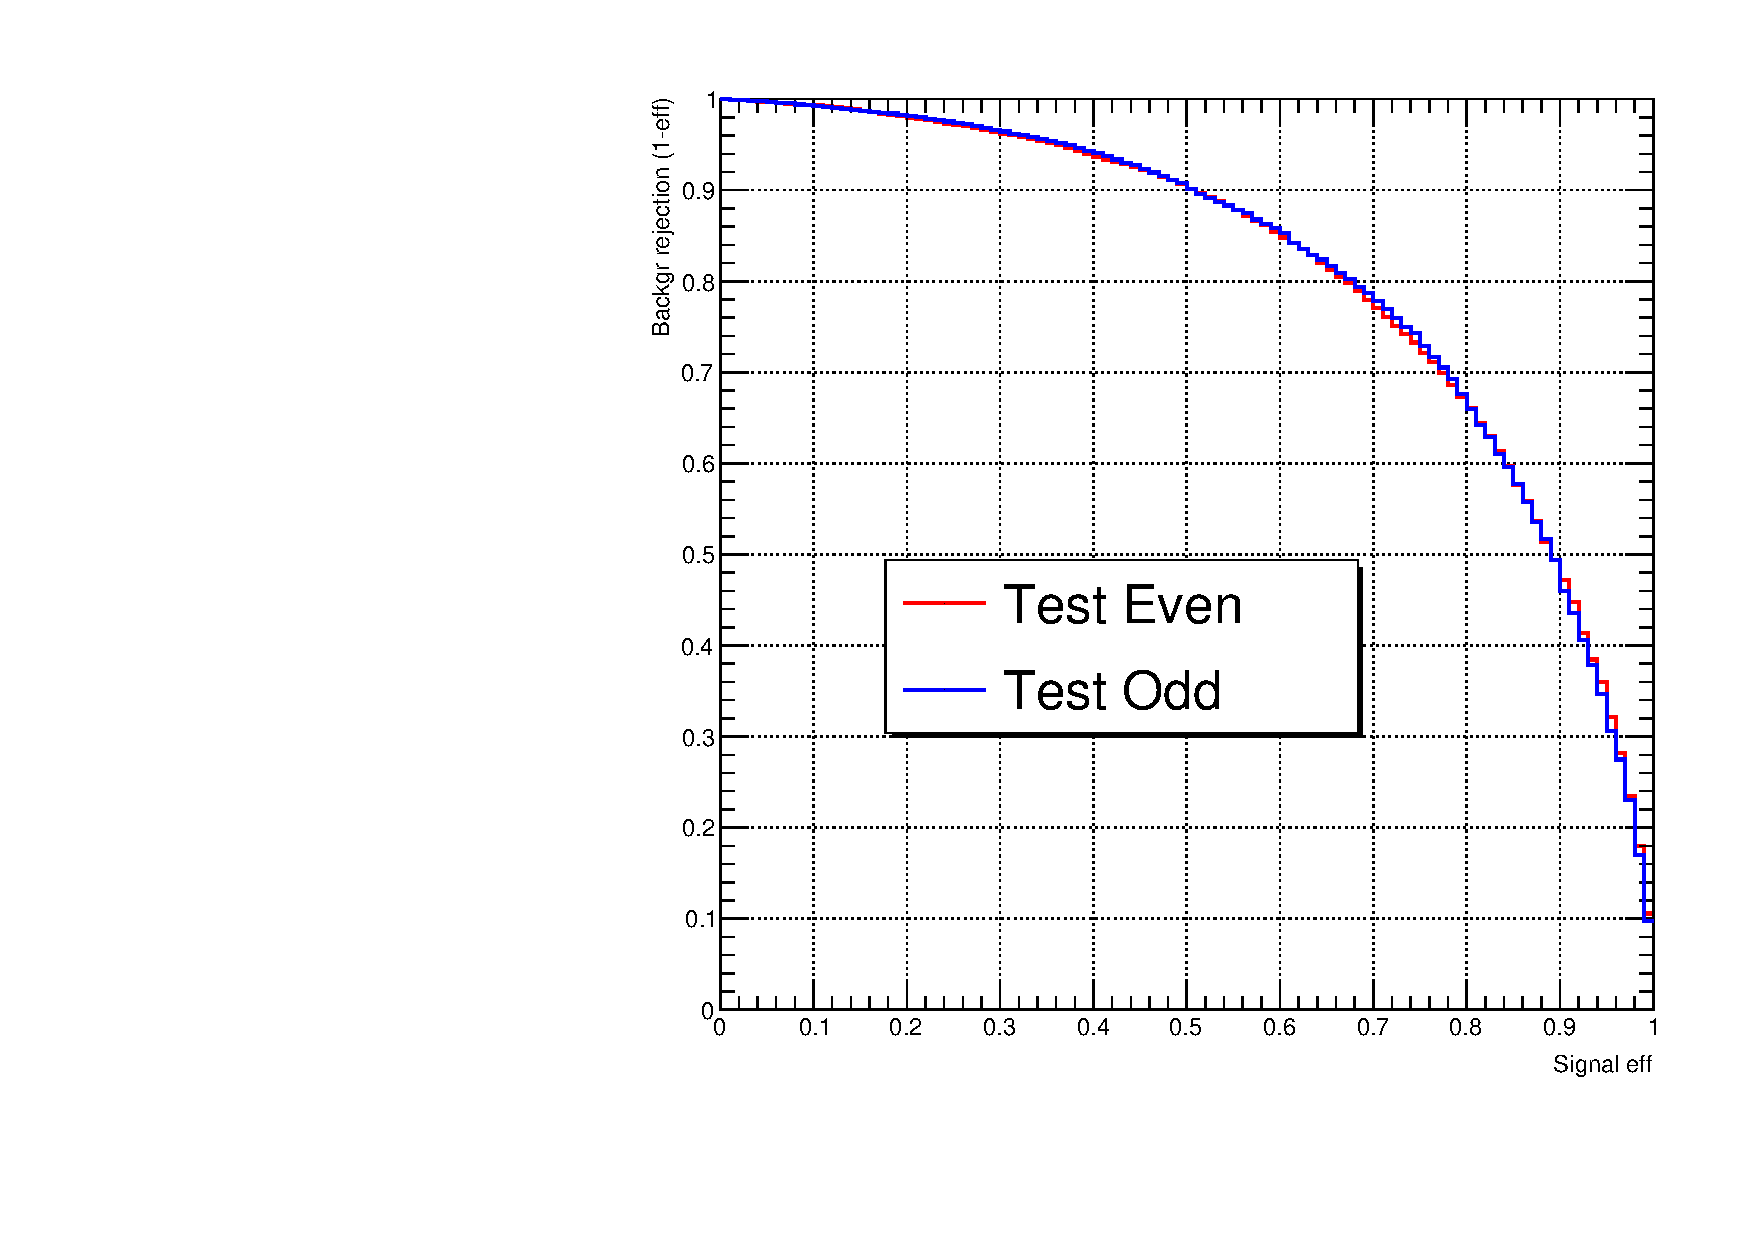
\includegraphics[width=0.33\textwidth]{\FCNCFigures/tthML/BDT/roc_reg1l1tau1b1j_ss.pdf}
\put(-70, 85){\textbf{(b3)}}\\

\includegraphics[page=4,width=0.33\textwidth]{\FCNCFigures/tthML/showFake/faketau/postfit/NOMINAL/reg1l1tau1b2j_ss_vetobtagwp70_highmet/BDTG_test.pdf}
\put(-40, 80){\textbf{(c1)}}
\includegraphics[page=5,width=0.33\textwidth]{\FCNCFigures/tthML/showFake/faketau/postfit/NOMINAL/reg1l1tau1b2j_ss_vetobtagwp70_highmet/BDTG_test.pdf}
\put(-40, 80){\textbf{(c2)}}
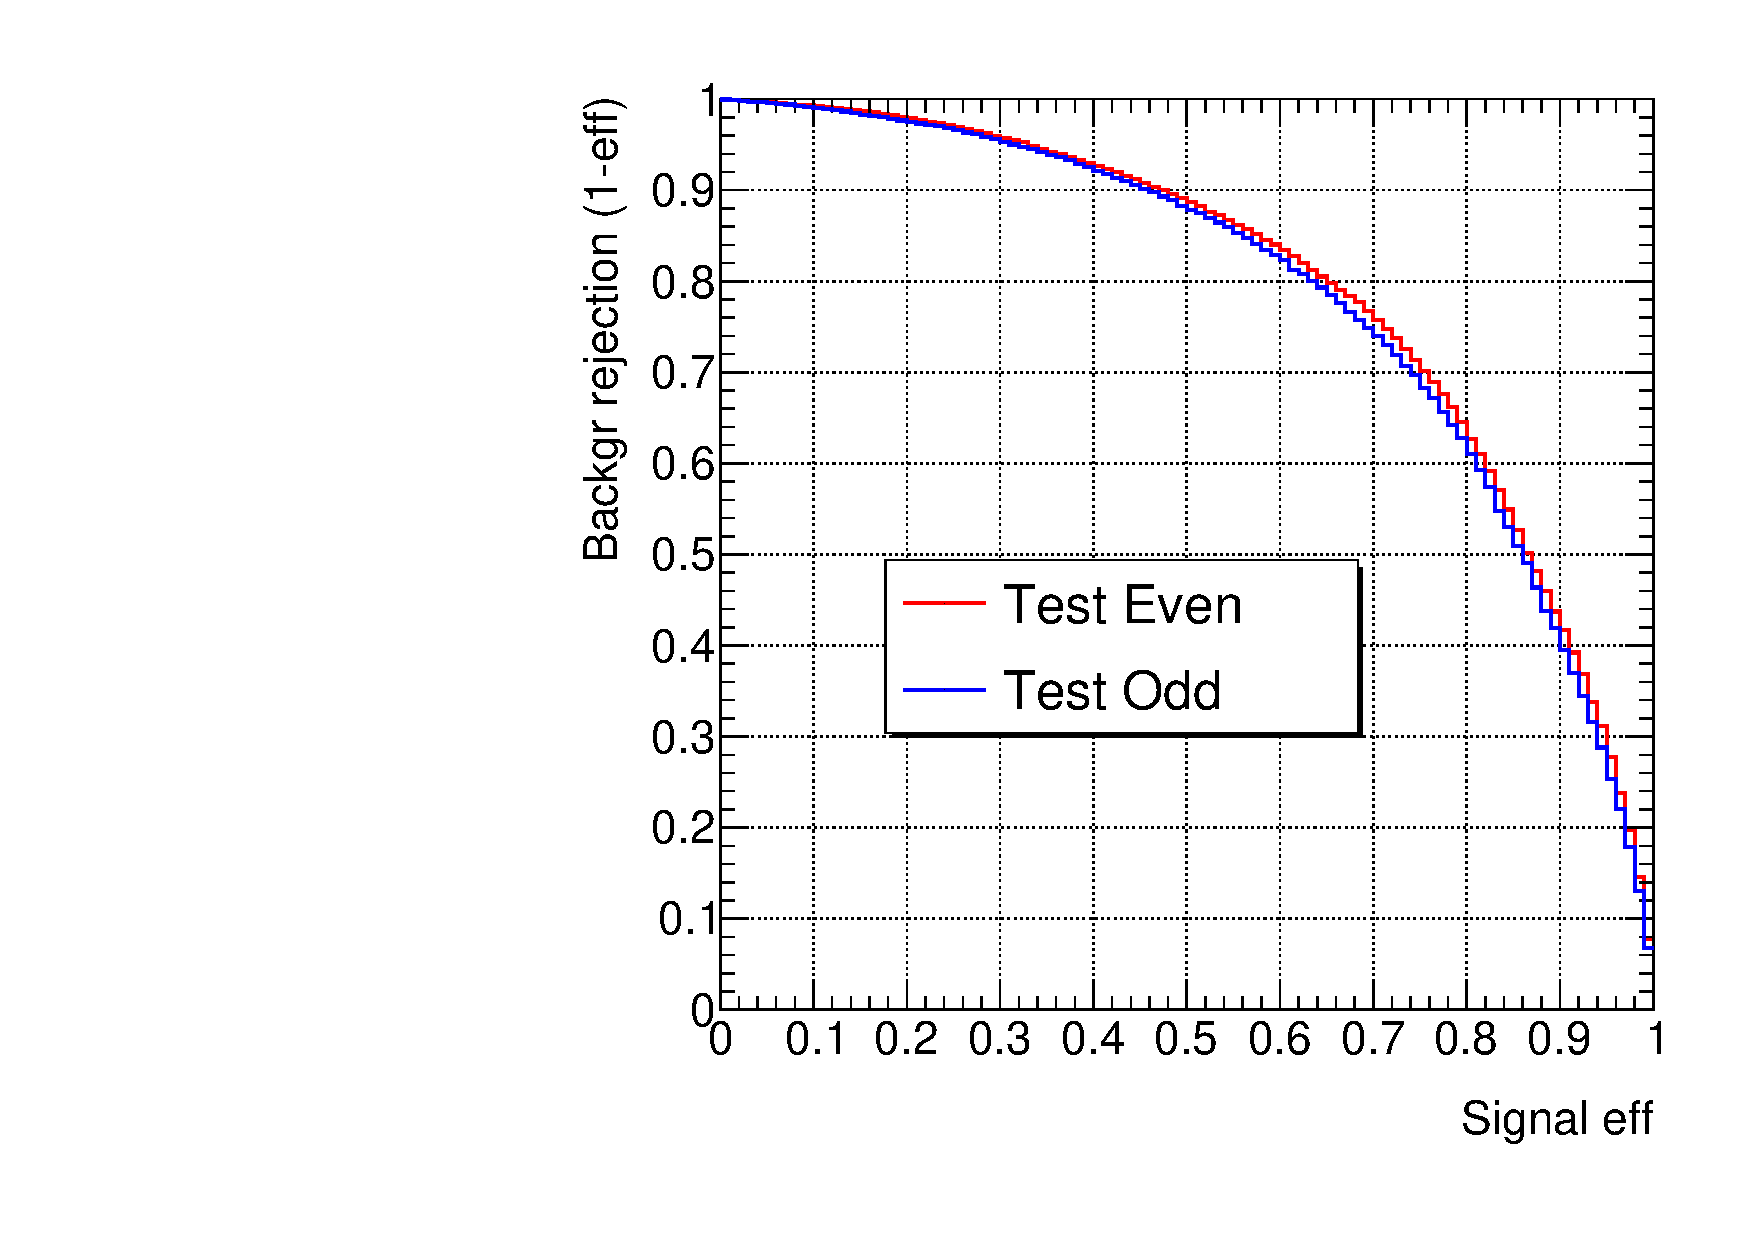
\includegraphics[width=0.33\textwidth]{\FCNCFigures/tthML/BDT/roc_reg1l1tau1b2j_ss.pdf}
\put(-70, 85){\textbf{(c3)}}\\

\includegraphics[page=9,width=0.33\textwidth]{\FCNCFigures/tthML/showFake/faketau/postfit/NOMINAL/reg1l2tau1bnj_os/BDTG_test.pdf}
\put(-40, 80){\textbf{(d1)}}
\includegraphics[page=9,width=0.33\textwidth]{\FCNCFigures/tthML/showFake/faketau/postfit/NOMINAL/reg1l1tau1b1j_ss_vetobtagwp70_highmet/BDTG_test.pdf}
\put(-40, 80){\textbf{(d2)}}
\includegraphics[page=9,width=0.33\textwidth]{\FCNCFigures/tthML/showFake/faketau/postfit/NOMINAL/reg1l1tau1b2j_ss_vetobtagwp70_highmet/BDTG_test.pdf}
\put(-40, 80){\textbf{(d3)}}\\

\caption{ The BDT output distributions for the background and TT signal (a1, b1, c1), background and ST signal (a2, b2, c2), background and different types of signals (d1,d2,d3) and ROC curves (a3, b3, c3) in the $t_l\thadhad$ (a1-3,d1), $t_l\tauhad$-1j (b1-3,d2), $t_l\tauhad$-2j (c1-3,d3) regions of leptonic channel.Only statistical uncertainties are being shown. Underflow and overflow bins are included respectively in the first and last bins. Empty data bins here are always blinded based on our strategy. The real tau contributions shown from ttbar and other MC including diboson, single top, and V+jets. }% The Kolmogorov Test values for the training and testing BDT distributions are also indicated.
\label{fig:overtrain_lhadhad}
\end{figure}

